\fancychapter{Laboratory results}
\label{chap:lab_res}

Following the design and simulation stages, a prototype was manufactured and assembled. However, practical implementations may differ from simulation results, as simulations generally rely on idealized component models and do not fully account for parasitic effects associated with the components and the \ac{pcb}. Therefore, laboratory testing was conducted to experimentally validate the design and verify that the prototype operates as expected.

\section{Design and assembly}

    AAll boards developed as part of this project, shown in Figure~\ref{fig:prototypes}, were designed using Altium Designer, manufactured by Eurocircuits, and assembled by hand to minimise production costs. The total cost of the electronic components is approximately 90~€, although this value may vary depending on the quantities purchased. The \ac{pcb} manufacturing cost ranges from approximately 3~€ to 35~€, depending on the manufacture.

    Consequently, the total cost of a complete prototype is approximately 125~€, which is lower than the cost of the product currently in use. Furthermore, the effective cost can be further reduced through component and manufacturing sponsorships.

    \begin{figure}[!ht]
        \centering
        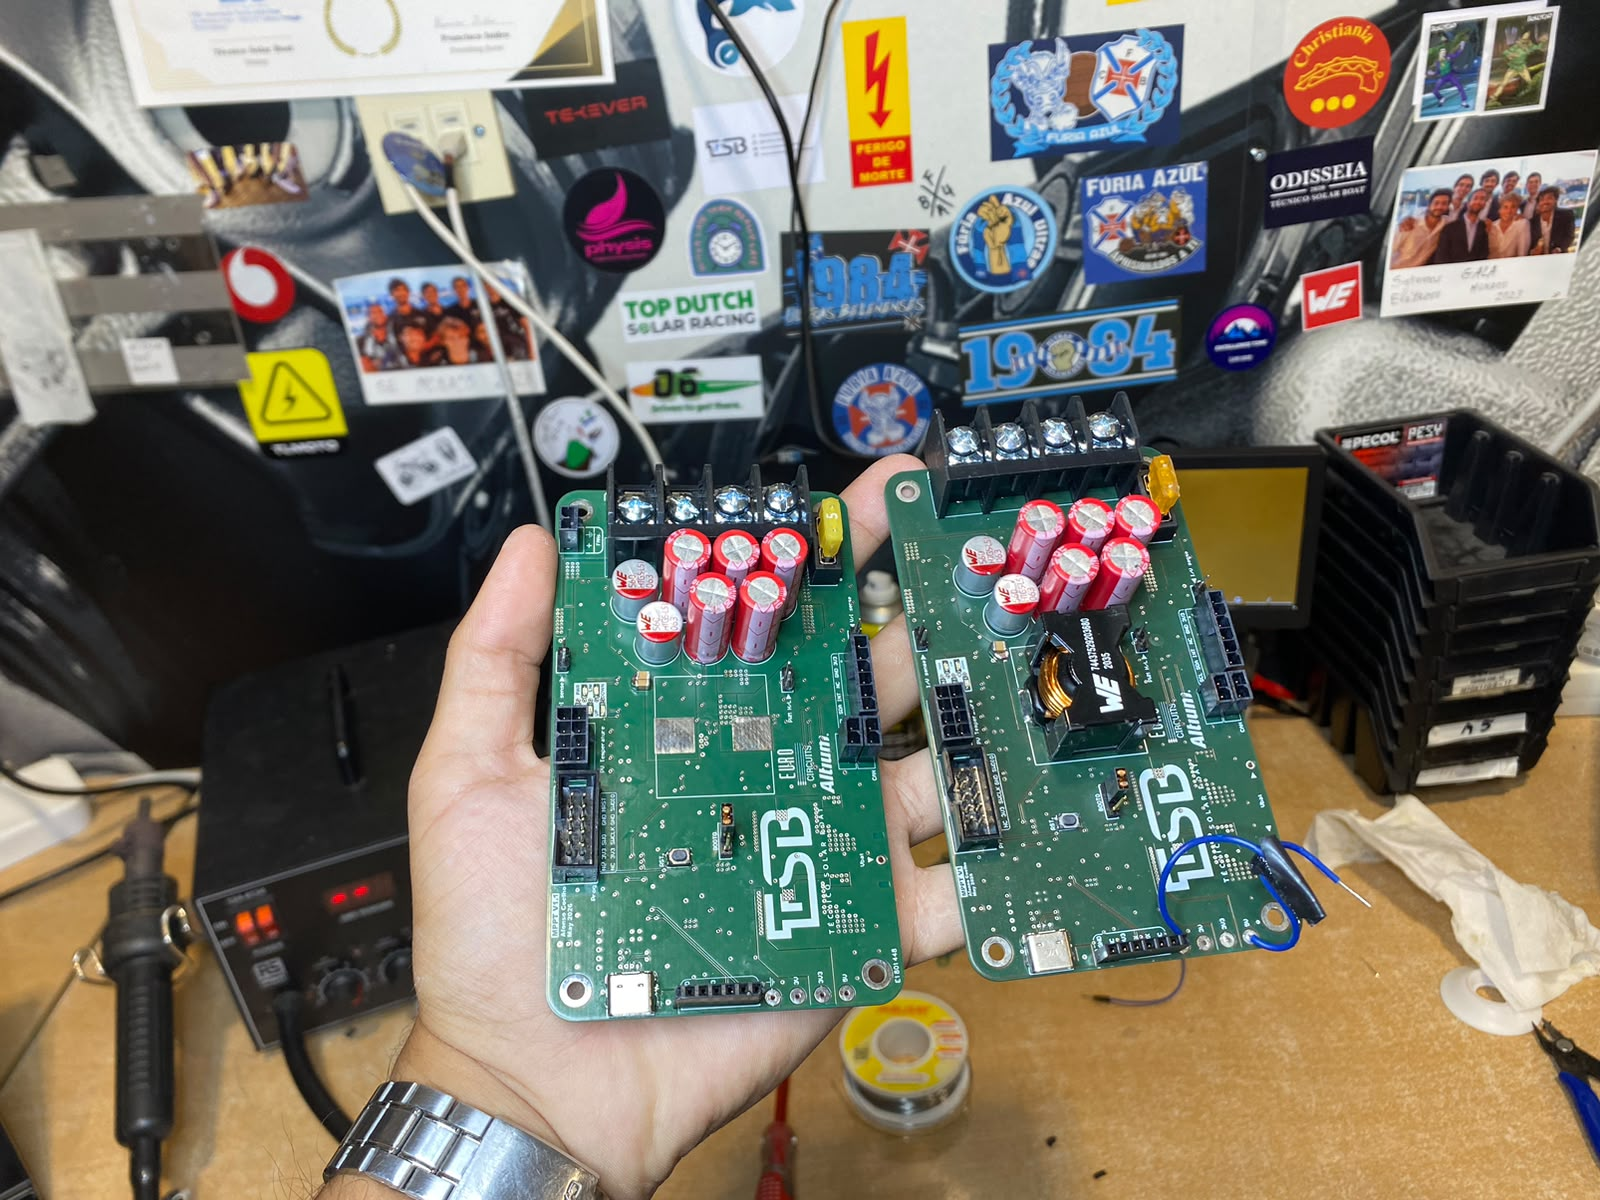
\includegraphics[width=0.6\textwidth]{Images/LAB_res/PCBsV1.1_1.2.jpeg}
        \caption{First and second iteration side by side. \textcolor{red}{place a better image}}
        \label{fig:prototypes}
    \end{figure}

    The \textbf{first prototype (V1)} iteration presented several issues that were identified during the initial testing phase. For instance, an incorrect 3D model resulted in the main connector being positioned incorrectly (Figure~\ref{fig:prototypes}).
    Additionally, the flash connector did not provide 5V which made test more difficult. The UART signals connected to the usb-c connector were swapped, and therefore the communication was only possible using a external USB to UART adapter. 

    Although none of these issues were critical for the fundamental operation of the circuit, they made the testing phase more time  consuming and complex. Therefore, a second iteration was designed and manufactured with all the issues fixed. 

    Besides the errors found in the first prototype, the \textbf{second iteration (V1.1)} two schottky diodes were placed in parallel with the boost transistors which accordingly to the datasheet of the transistors, should improve the efficiency of the boost converter. After some simulations, if was found that this statement does not aplie in this case due to the short deadtime. Furthermore, during testing of the first iteration, an increase in the inductor temperature was observed. To address the possibility of requiring additional cooling,  a connector was added to place a fan if needed. These will also be analyzed in this section.

    Near the end, a \textbf{final version (V1.2)} was made, which includes the extra filter capacitors to filter noise which will be discussed later. Additionally, the sensors filters were placed near the sensors. Since switching devices generate electromagnetic noise, the filters should be close to the \ac{mcu} pins.  

    Due to time constraints, the majority of the results presented in the following sections were obtained using version V1.1. Whenever results obtained with the latest version are presented, this will be explicitly stated, otherwise, the results refer to version V1.1.


\section{Voltage and Current sensor}
    Both current and voltage sensors were tested in the laboratory to validate the performance and accuracy of the measurements. 

    The voltage sensor test was performed by applying a known voltage to the input and measuring MCU readings. 

    The test was performed over the entire voltage range required for the application, from $0$~V to $51$~V. The results demonstrate that the voltage sensors provide accurate measurements, with average absolute errors of $60$~mV for the battery voltage measurement and $112$~mV for the solar panel voltage measurement. The error is different for each sensor because it depends on the actual resistance of the resistors used in the voltage dividers and the \ac{pcb} layout. For each board the error will be different, but it is expected to be in the same order of magnitude since the tolerance of the resistors are equal.

    These could be improved even further by using resistors with less tolerance and lower temperature coefficient or by increasing the ADC resolution. Another option that does not increase the cost of the system is to subtract the linear error of the results. The magnitude of the error is small, and therefore it does not affect the \ac{mppt} operation, however, for the purpose of this project, the linearization was implemented in firmware to improve the accuracy of the measurements made during the testing phase.

    In Figure~\ref{fig:voltage_sense_error} the error of the voltage readings is represented. Since the error is linear, the trend line is also represented, which was used to correct the results and improve the accuracy of the measurements. The results after subtracting the linear error are also represented in the figure, and it can be seen that the error is significantly reduced. The average error reduced to 28.325~mV and 29.825~mV for battery and solar panel respectively. 

    \begin{figure}[!ht]
        \centering
        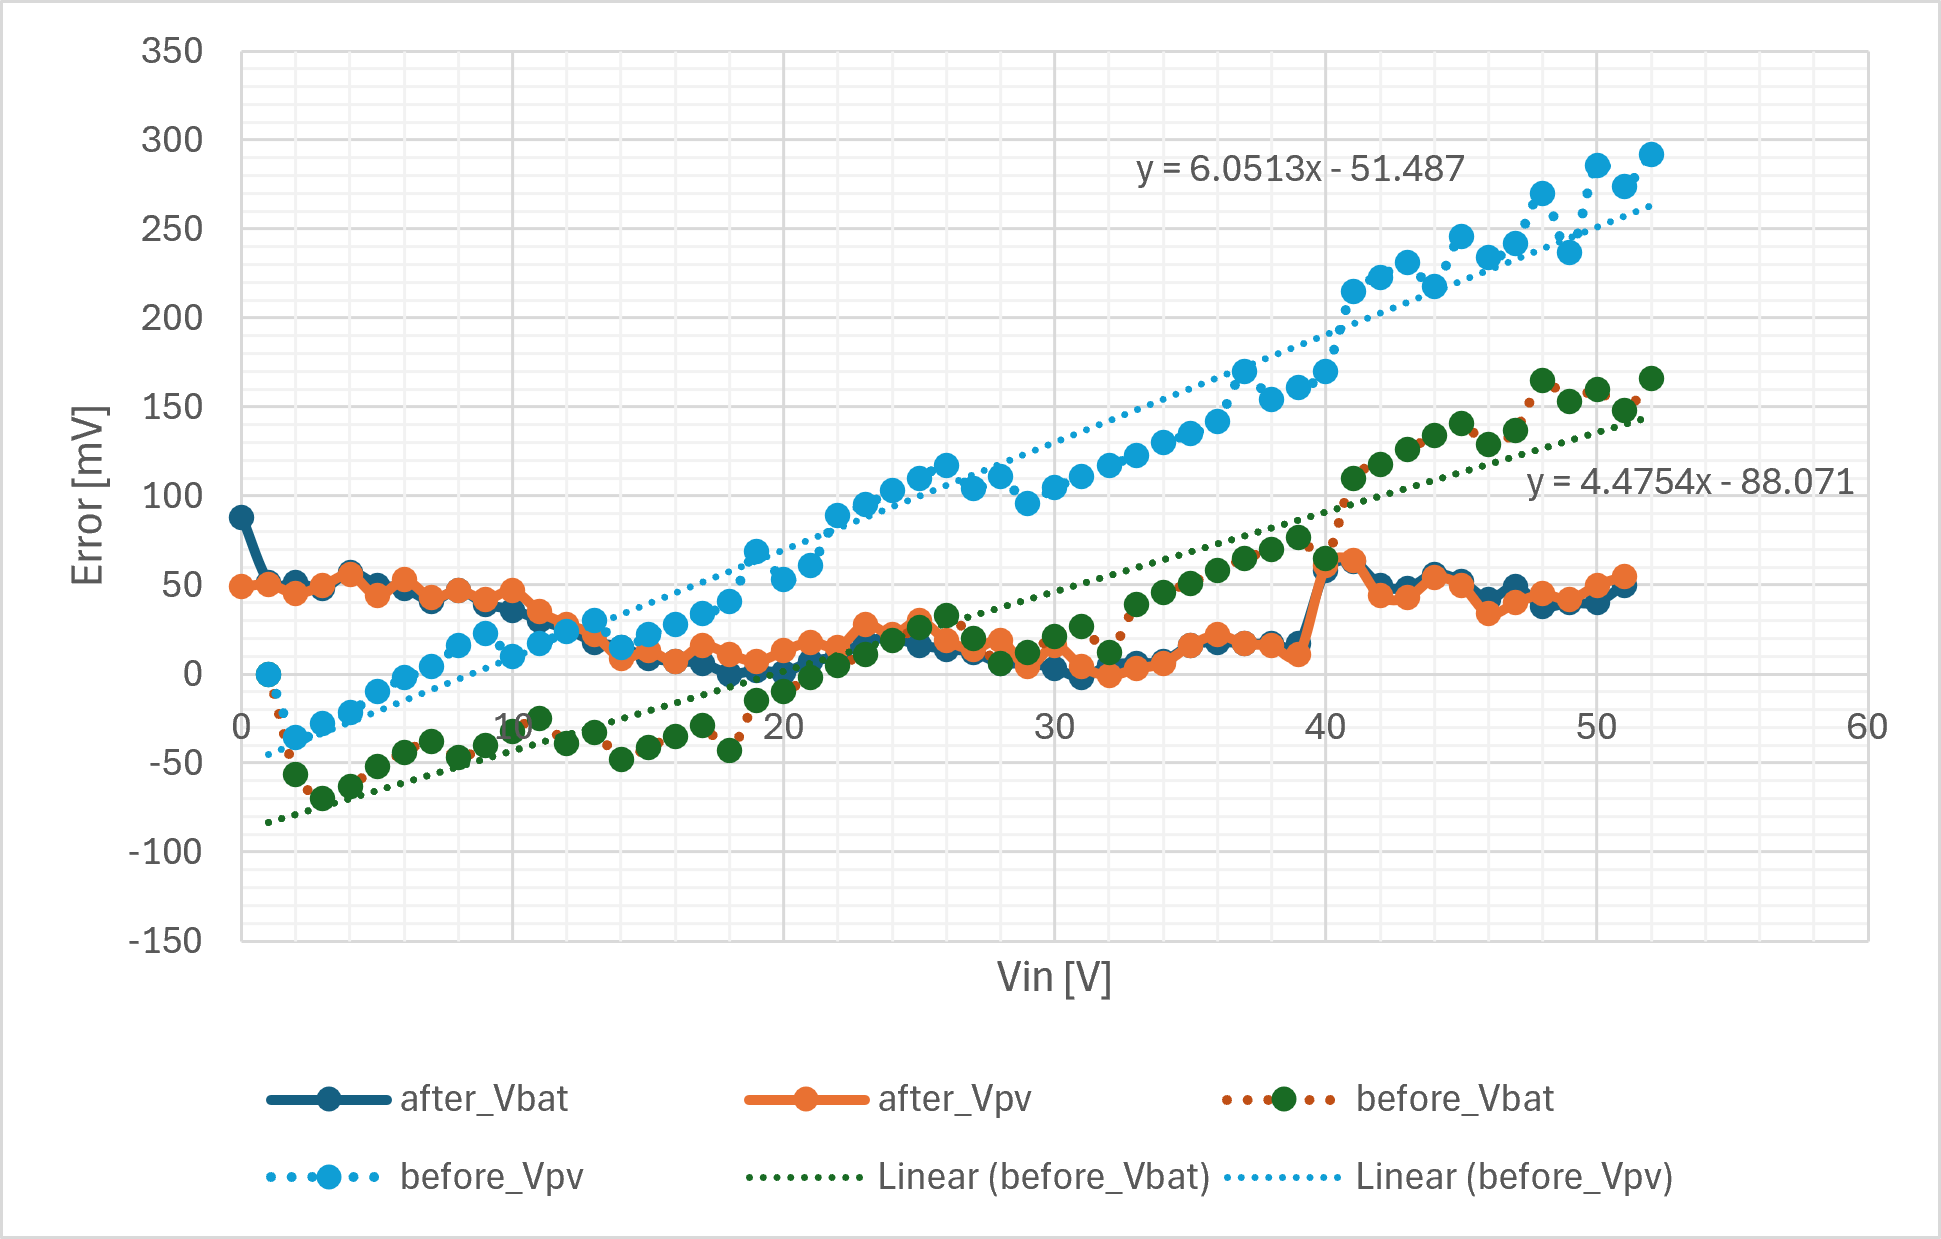
\includegraphics[width=0.6\textwidth]{Images/LAB_res/Voltage_sensor_test.png}
        \caption{Voltage sensor error over voltage.}
        \label{fig:voltage_sense_error}
    \end{figure}

    The same test was performed for the current sensors, the average error was 99.93~mA and 8.5~mA for battery and solar panel respectively, which is acceptable for this application. The error of the current sensors is shown in Figure~\ref{fig:current_sense_error}, and it can be seen that the error is linear for the battery side and non-linear for the solar panel side. This can be explained by the fact that at low currents, the error is smaller and probably the shunt resistor value in the solar panel side is more accurate than the shunt resistor in the battery side. However, it is still small and does not affect the \ac{mppt} operation.

    As in the case of the voltage sensor, the subtraction of the linear error would highly increase the accuracy of the measurements. However, it takes a lot of time to do the measurements and calculate the linearization for each \ac{pcb} which is not realistic for a student prototype project like \ac{tsb}. However, to increase the accuracy of the laboratory results, the error correction was implemented to the battery side current sensor. The results after subtracting the linear error are also represented in the figure, and it can be seen that the error is significantly reduced. The average error reduced to 5.28~mA.

    \begin{figure}[!ht]
        \centering
        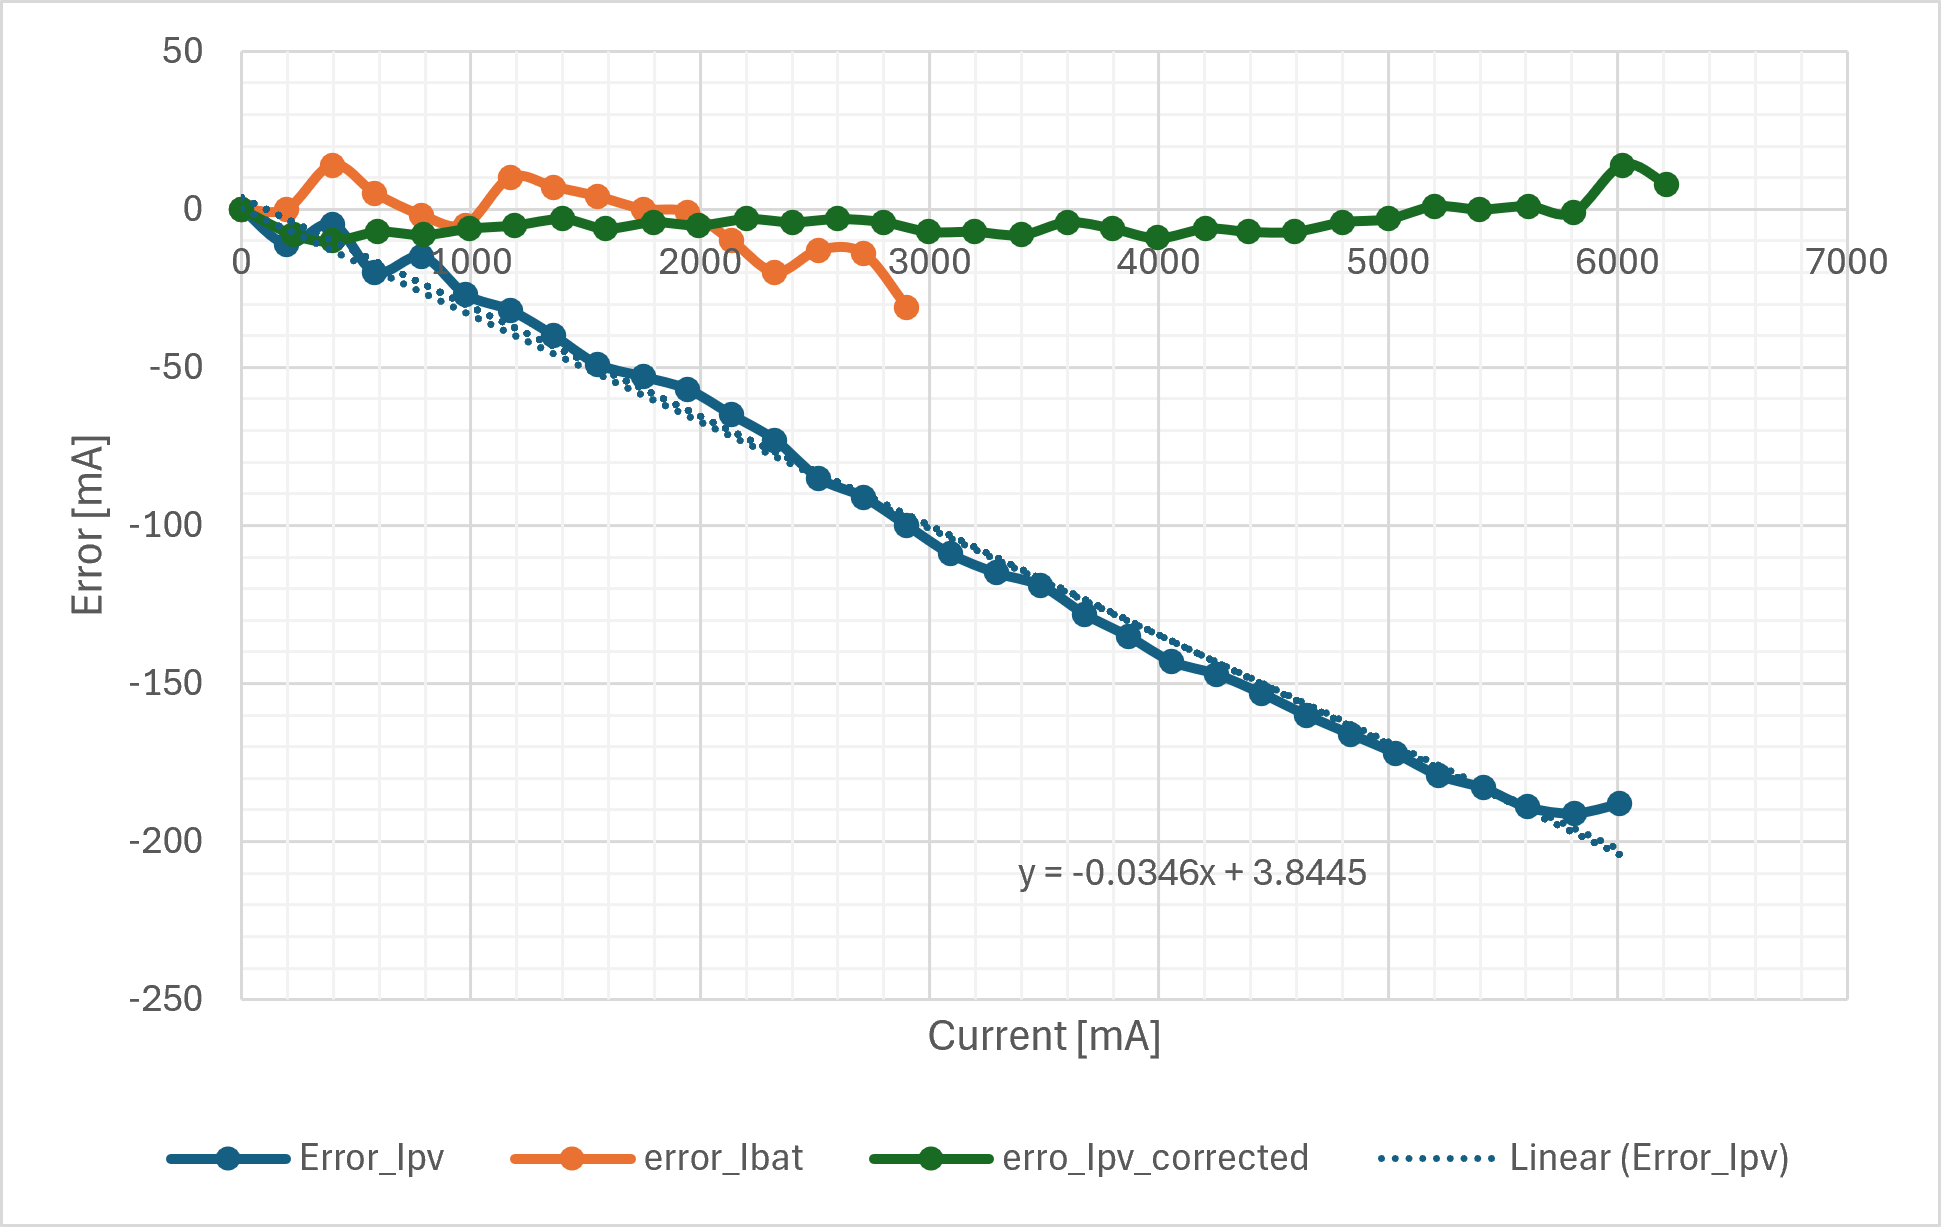
\includegraphics[width=0.6\textwidth]{Images/LAB_res/Current_sensor_test.png}
        \caption{Current sensor error over current.}
        \label{fig:current_sense_error}
    \end{figure}


\section{Boost}
    The Boost test is essential to identify the efficiency and the correct operation of the synchronous boost converter without the influence of the control system. Additionally, it is essential to confirm the correct dimensioning of the power converter enabling a comparison with simulations and theoretical calculations.

    The test was performed using a voltage source on the input side and two power resistors on the load side. Both duty cycle and load resistance were varied to obtain the results in all different points of the charging curve, Figure~\ref{fig:cc-cv points}.

    All the measurements were performed with multimeter with high precision. The voltage readings were performed as close as possible to the \ac{pcb}, as for the current readings, they have to be performed in line.

    It is important to note that this board uses the battery side to power itself, however in this test the battery side is not connected to a battery but since the \ac{pv} side is connected to a voltage source, this energy flows to the battery side through the boost converter diodes/body diodes and therefore powering the control system.
        
    \subsection{Switching noise}
        \textcolor{red}{This subsection will be rewritten with results from V1.2. The idea is to caracterize the noise with a spectrum analayzer and compare with CISPR 25 regulation (regulations for conductive EMI measurement).}

        During the initial experimental tests, a significant amount of electrical noise was observed in all measured signals. The measured noise caused the current to exceed the configured \ac{oc} protection thresholds, resulting in repeated activation of the protection mechanism. Initially, it was assumed that the problem originated from the \ac{pcb} measurement system. Consequently, several modifications were implemented in the firmware, mainly increasing the ADC sampling time and increasing the number of samples acquired for each measurement, with the final measurement being obtained by averaging the collected samples. Furthermore, the fault handling logic was modified, because once a \ac{oc} fault occurred, the converter entered an oscillatory state in which it repeatedly enabled and disabled itself. Now when a fault occurred, it waits 1 second and verifies if the fault was removed. Although these software modifications improved the stability and accuracy of the measurements, they did not eliminate the excessive noise.

        During the \ac{oc} events, a large oscillation in the input current was also observed, varying approximately between 4~A and 12~A. One possible explanation considered was that the laboratory power supply was operating close to its current limit, causing it to become unstable. Replacing the power supply was therefore considered as a potential solution. However, since the observed noise was considerably higher than expected, it was believed that the root cause was located elsewhere.

        A detailed analysis of the reference evaluation board revealed a significant difference in the output decoupling network. While the initial prototype employed a single 1~$\mu$F ceramic capacitor, which completely eliminated the switching noise in simulation, the reference evaluation board used ten 1~$\mu$F ceramic capacitors connected in parallel.

        To evaluate the impact of the output capacitance, the converter was characterized without any changes. Figure~\ref{fig:ruido inicial} shows the initial noise.

        In all oscilloscope captures, Channel~1 (yellow) corresponds to the output current ($I_{out}$), Channel~2 (blue) to the input voltage ($V_{in}$), Channel~3 (orange) to the input current ($I_{in}$), and Channel~4 (green) to the output voltage ($V_{out}$). Although the screenshots are not of optimal quality, they clearly illustrate the reduction in switching noise obtained after increasing the output decoupling capacitance.

        To increase the local output decoupling, nine additional 1~$\mu$F ceramic capacitors were soldered in parallel with the existing capacitor, matching the total capacitance used in the evaluation board. After this modification, a significant reduction in the measured noise was observed, as shown in Figure~\ref{fig:ruido final}.

        These results confirm that the insufficient output decoupling capacitance was the primary contributor to the observed electrical noise. Increasing the number of ceramic capacitors substantially improved the converter performance and reduced measurement fluctuations. 
        
        Although the results were already satisfactory, the reference evaluation board also includes seven additional 220~nF ceramic capacitors distributed across the output stage. Initially the board also had one smaller capacitor (100~nF) and since it was not possible to get 220~nF with 100~V rating, a six 100~nF capacitors were added. The result should be similar. These capacitors are expected to further reduce the high frequency switching noise. The results are presented in Figure~\ref{fig:ruido final 2}.

        The approximate peak noise amplitudes measured for each hardware configuration are summarized in Table~\ref{tab:noise_comparison}. Adding nine 1~$\mu$F ceramic capacitors significantly reduced both the current and voltage noise. Subsequently, the six additional 100~nF ceramic capacitors further reduced the current noise, although the input voltage increased but it may be due to imprecise measurements from the oscilloscope. x

        \begin{table}[!ht]
            \centering
            \caption{Approximate noise amplitudes measured for the three hardware configurations. \textcolor{red}{I do not like how these values were measured. In reality the values are less than a quarter. They must be measured separately with a good trigger. I may redo it in V1.3. }}
            \label{tab:noise_comparison}
            \begin{tabular}{|l|cccc|}
                \hline
                Quantity &
                Original &
                +9 $\times$ 1~$\mu$F &
                +9 $\times$ 1~$\mu$F +6 $\times$ 100~nF &
                ...+ schottky diode\\
                \hline
                $I_{in}$  & 1.8 A   & 640 mA & 292 mA & 140 mA \\
                $I_{out}$ & 0.8 A   & 300 mA & 220 mA & 272 mA \\
                $V_{in}$  & 2.0 V   & 350 mV & 380 mV & 490 mV \\
                $V_{out}$ & 8.0 V   & 2.3 V  & 2.2 V  & 1.440 V \\
                \hline 
            \end{tabular}
        \end{table}

        \begin{figure}[!ht] 
            \centering 
            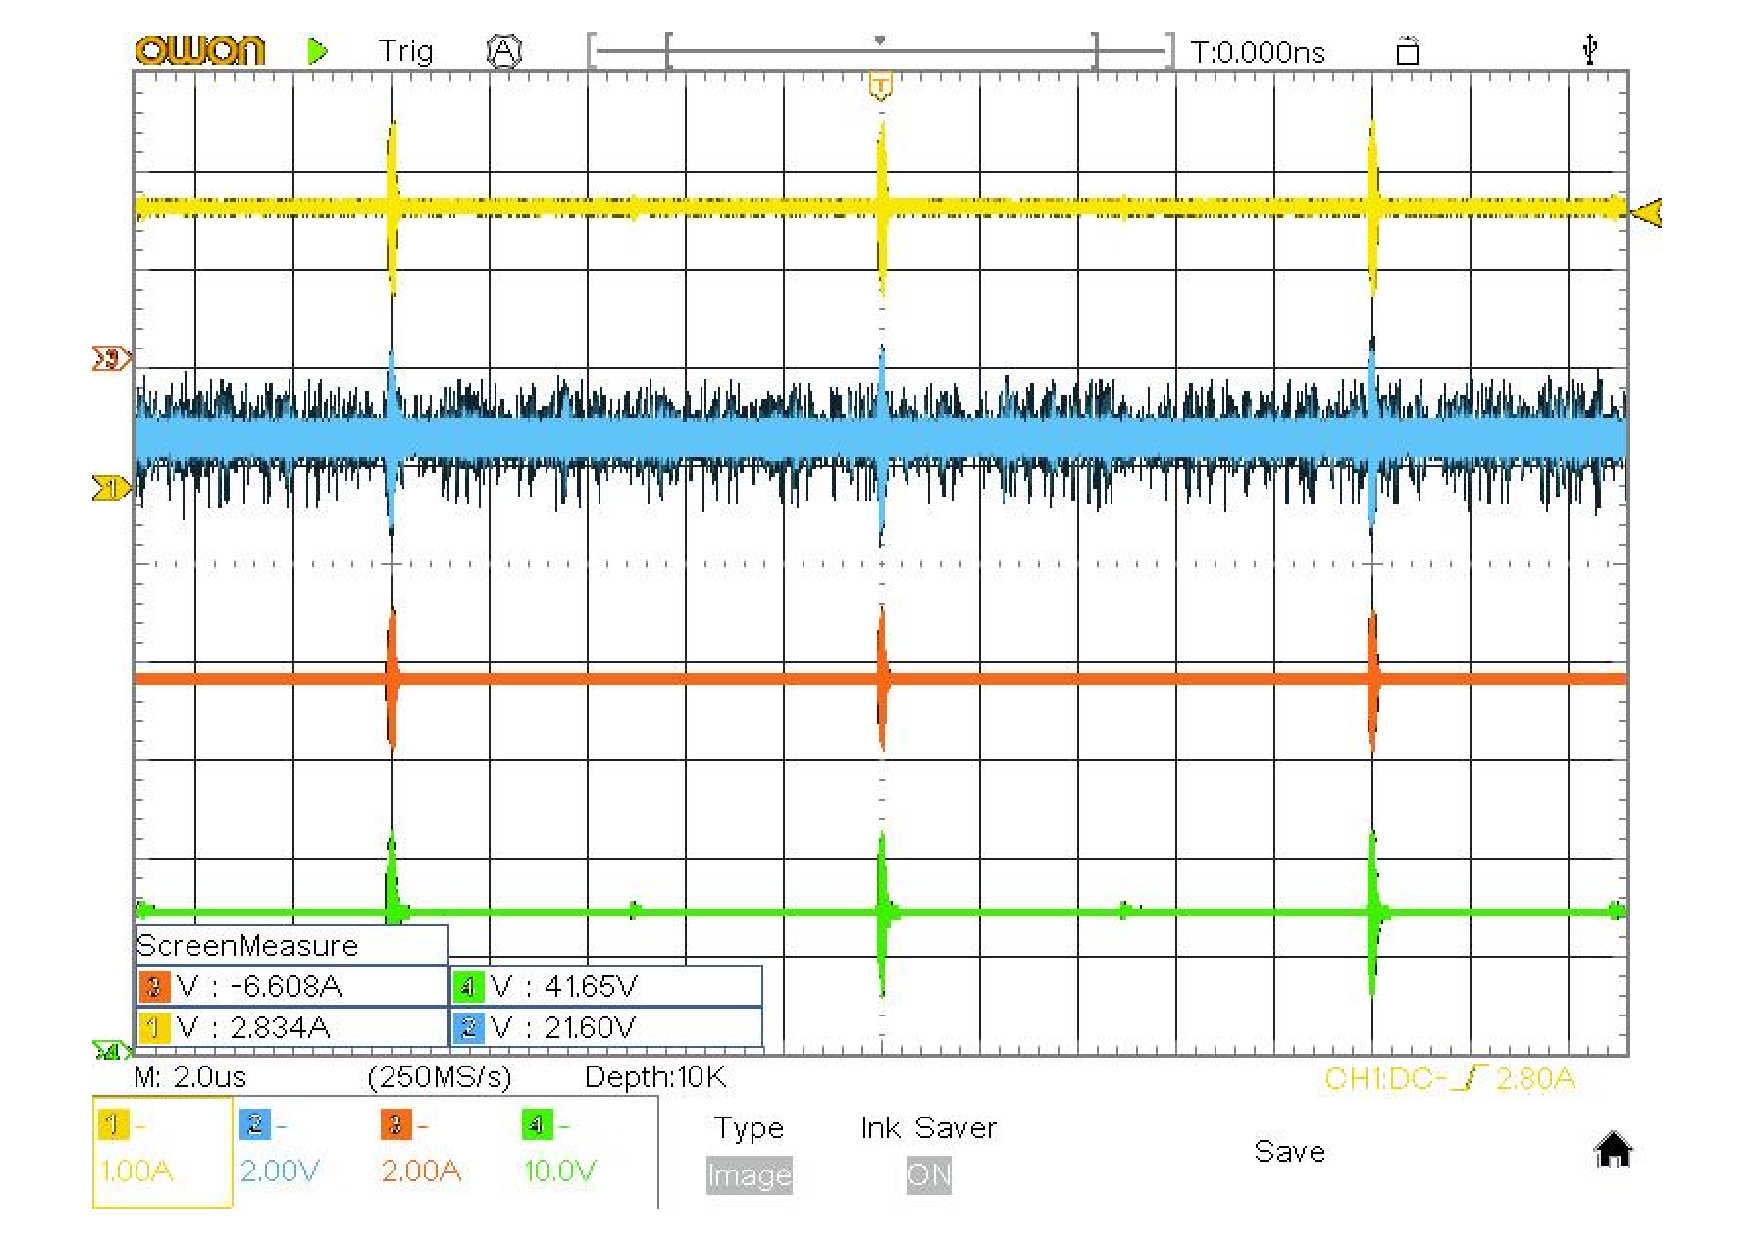
\includegraphics[width=0.6\linewidth]{Images/LAB_res/case2-1.pdf} 
            \caption{Measured waveforms before adding the additional ceramic capacitors.} 
            \label{fig:ruido inicial}
        \end{figure}

        \begin{figure}[!ht] 
            \centering 
            \begin{minipage}{0.49\textwidth}
                \centering 
                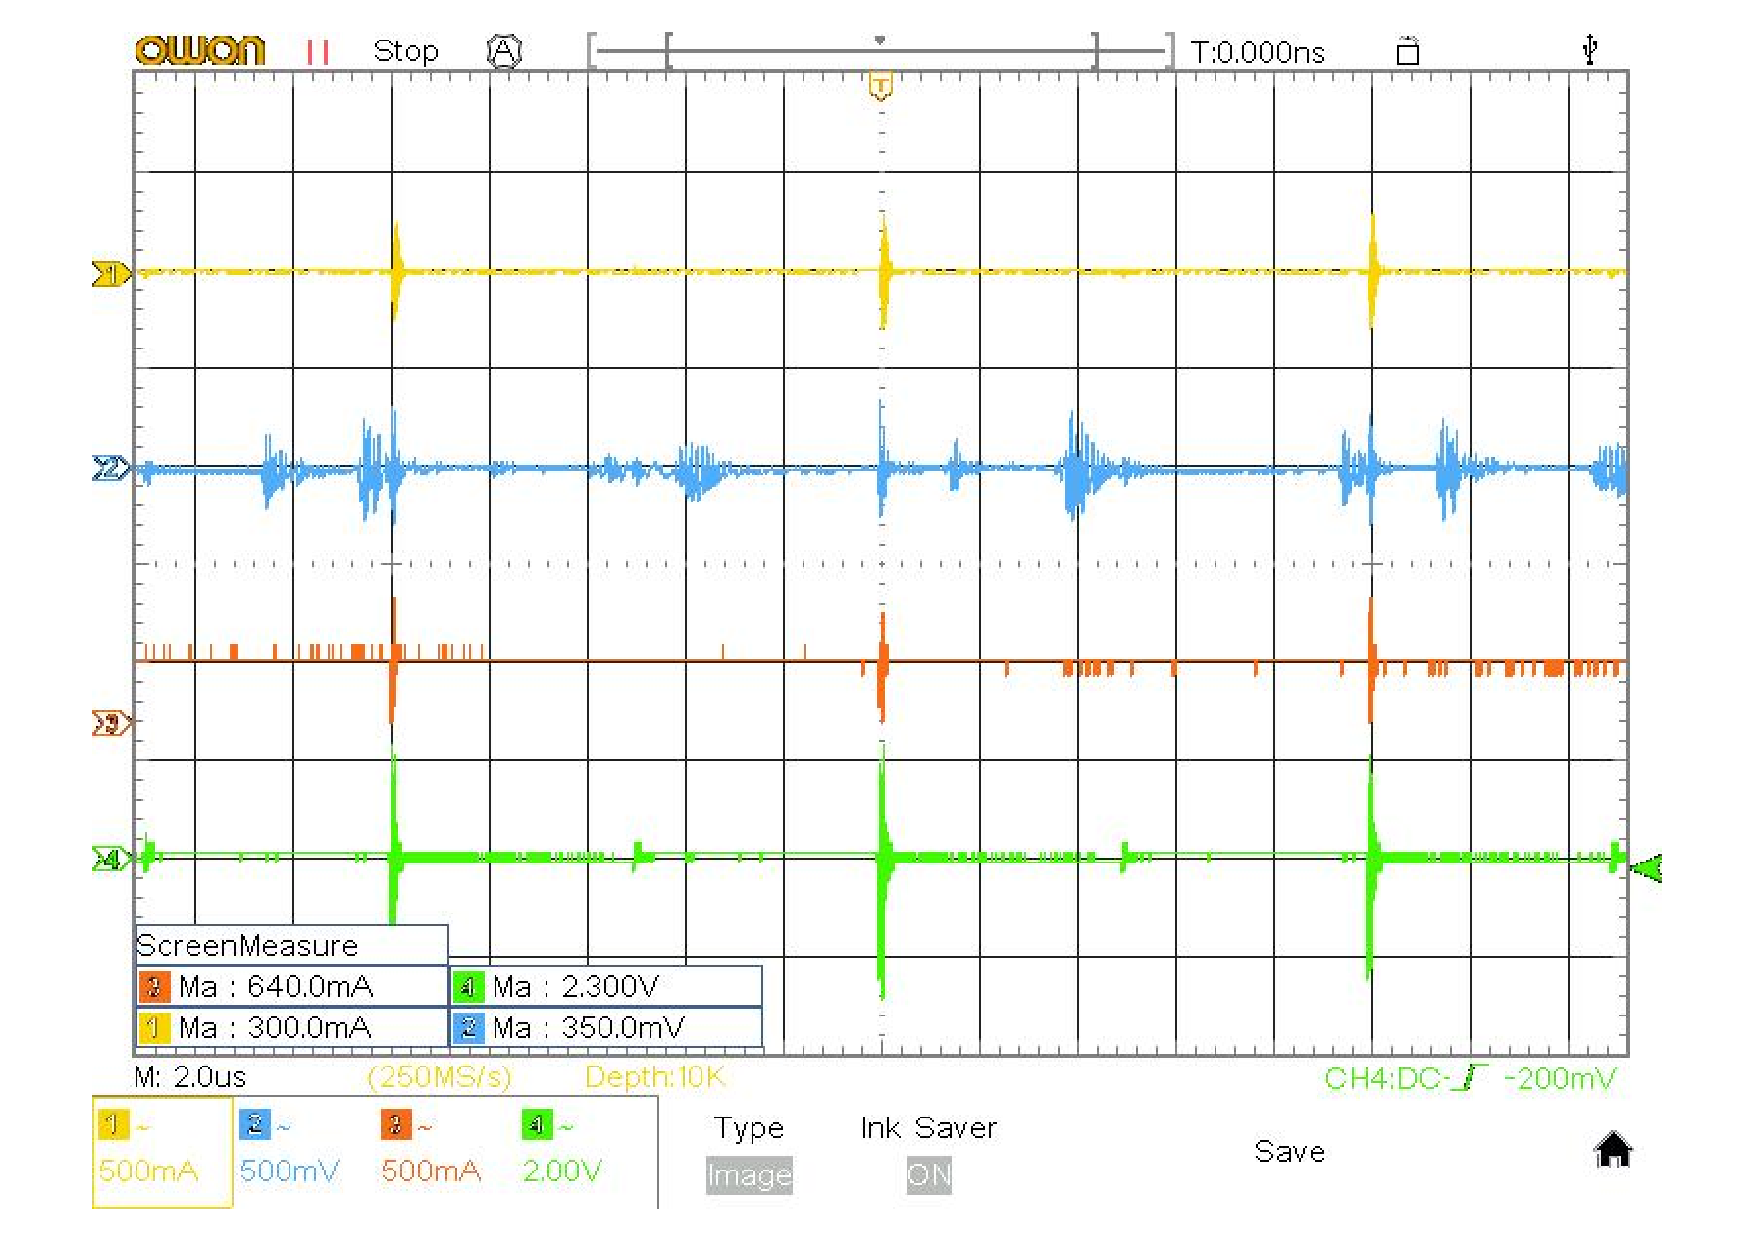
\includegraphics[width=\linewidth]{Images/LAB_res/case2-2.pdf}
                \caption{Measured waveforms after adding nine additional 1~$\mu$F ceramic capacitors.} 
                \label{fig:ruido final} 
            \end{minipage} 
            \hfill 
            \begin{minipage}{0.49\textwidth} 
                \centering 
                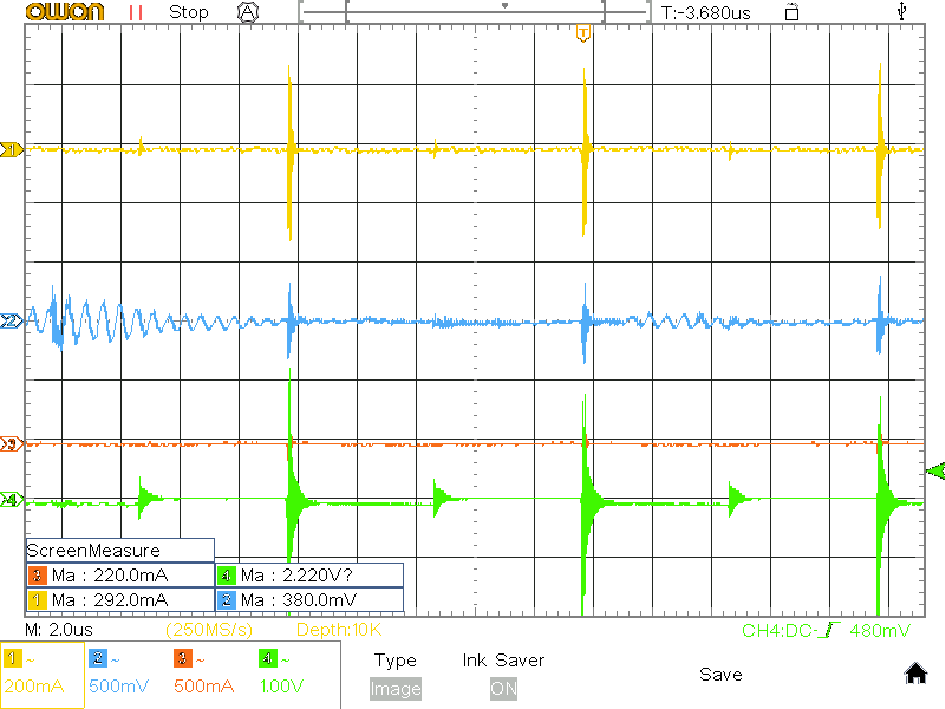
\includegraphics[width=0.9\linewidth]{Images/LAB_res/case2-3.pdf} 
                \caption{Measured waveforms after adding nine additional 1~$\mu$F ceramic capacitors.} 
                \label{fig:ruido final 2} 
            \end{minipage} 
        \end{figure}

    \subsection{Efficiency}
        The efficiency of the \ac{mppt} charger is one of the most important parameters to be measured since it directly affects the power that is effectively extracted from the solar panel and delivered to the battery. As in simulations, the efficiency was measured for each point of the charging curve. All the measurements were taken with the multimeter and the results are presented in Table~\ref{tab:efficiency_results}.

        \begin{table}[!ht]
            \centering
            \caption{Efficiency measurements for the different test cases.}
            \label{tab:efficiency_results}
            \begin{tabular}{|l|ccc|cc|}
                \hline
                & \multicolumn{3}{c|}{Multimeter} 
                & - OC power 
                & - OC+Transistors power \\
                \hline
                Case & Power in & Power out & Efficiency 
                & Efficiency & Efficiency \\
                \hline
                Case 1 & 127.444 & 123.413 & 96.84\% & 97.23\% & 97.64\% \\
                Case 2 & 129.108 & 124.685 & 96.57\% & 96.96\% & 97.36\% \\
                Case 3 & 127.523 & 123.232 & 96.64\% & 97.02\% & 97.43\% \\
                Case 4 & 73.1277 & 70.818 & 96.84\% & 97.52\% & 98.24\% \\
                \hline
                OC & 0.5103 & 0 & -- & -- & -- \\
                OC+Transistors & 1.04279 & 0 & -- & -- & -- \\
                \hline
            \end{tabular}
        \end{table}

        The measured efficiency is more than 96\% for all test cases, which is an extraordinary result. This efficiency takes into account all the losses in the converter, including the measurement system and control system. When compared with the power losses estimation made in section~\ref{subsubsec:loss_estimation}, the efficiency is around 2\% lower than expected. This difference can be explained by the fact that the components used can have slightly different characteristics. Also, the losses caused by the parasitic elements of the \ac{pcb} were not considered in the estimation.

        The \ac{pcb} was also tested in open circuit with and without driving the transistors. The results show the losses of the circuit without the boost converter. Around 0.5~w of losses are caused only by the measurement and control system. When the transistors are driven without any load, the loses of the converter are negligible since the current is too low. So the measured losses are approximately equal to the driving circuit + the measurement and control system. Based on these values, in table~\ref{tab:efficiency_results} it is also present a estimate of the efficiency without the measurement and control system and another without the driving circuit too. The converter efficiency is around 97\% to 98\% for all test cases, which is close to the simulation measurements. From another perspective, it shows just how significant the losses are on the rest of the circuit.         

    \subsection{Temperature rise}
        The temperature of each element was measured before each test and after 10 min. All test show similar result, a temperature rise of up to 10ºC. The inductor is the main heat element, reaching 43ºC, the capacitors also reach around 40ºC hover they are placed side by side with the inductor which heats the capacitors. As expected, the transistors do not overheat. The maximum temperature measured was 39.5ºC. 

        The results are close to what was expected. In Section~\ref{subsubsec:loss_estimation}, we concluded that the component with the highest losses is the inductor, followed by the transistors and the capacitors. In this section, it is expected that the temperature follows the same order since it is related to the losses. However, the measurements do not follow the expected results. This is explained by the fact that each of these components have different surface areas, and therefore there heat dissipation is not comparable. 

        Thermal images of the circuit were also obtained, as shown in Figures~\ref{fig:thermal_front} and \ref{fig:thermal_back}, allowing the areas with the highest temperatures to be identified. However, the quality of the images is limited, and a vertical offset can be observed between the thermal and visible images. Furthermore, the vertical lines present in the thermal images are measurement artefacts caused by the thermal imaging device and do not represent actual temperature variations.

        Despite these limitations, the results indicate that the inductor is the component reaching the highest temperature, with a noticeable spread of heat to the surrounding area. The capacitors also exhibit some heat dissipation, although at a lower magnitude than the inductor. On the rear side of the PCB, the only components showing a significant increase in temperature are the transistors.


        \begin{figure}[!ht] 
            \centering 
            \begin{minipage}{0.49\textwidth}
                \centering 
                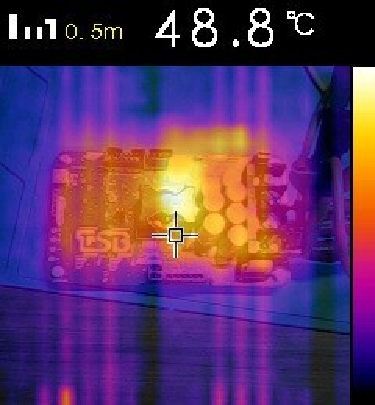
\includegraphics[width=0.9\linewidth]{Images/LAB_res/IMG00029.pdf} 
                \caption{Front side thermal image.} 
                \label{fig:thermal_front} 
            \end{minipage} 
            \hfill 
            \begin{minipage}{0.49\textwidth} 
                \centering 
                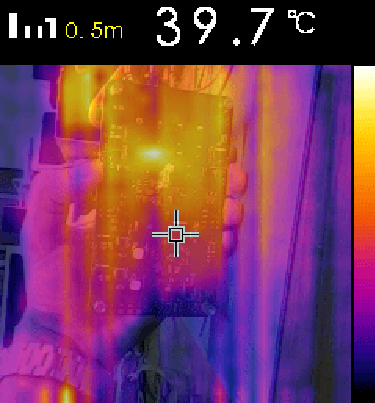
\includegraphics[width=0.9\linewidth]{Images/LAB_res/IMG00030.pdf} 
                \caption{Back side Thermal image.} 
                \label{fig:thermal_back} 
            \end{minipage} 
        \end{figure}

        To confirm that the temperature does not rise to a concerning level, a test of 3 hours was performed with the converter operation at Case 3. In figure~\ref{fig:3h_temp_test} it is represented the temperature evolution over the 3 hours for the inductor, capacitors, transistors and the ambient temperature. These results were acquired using the thermistors placed on the board which measure the ambient temperature and the transistors temperature. The other measurements where acquired using additional external thermistors that can read by the board using the connector placed for thermistors. 

        The measured values were confirmed using an infrared thermometer which show insignificant different temperature, confirming the quality of the measurements.
        
        \begin{figure}[!ht] 
            \centering 
            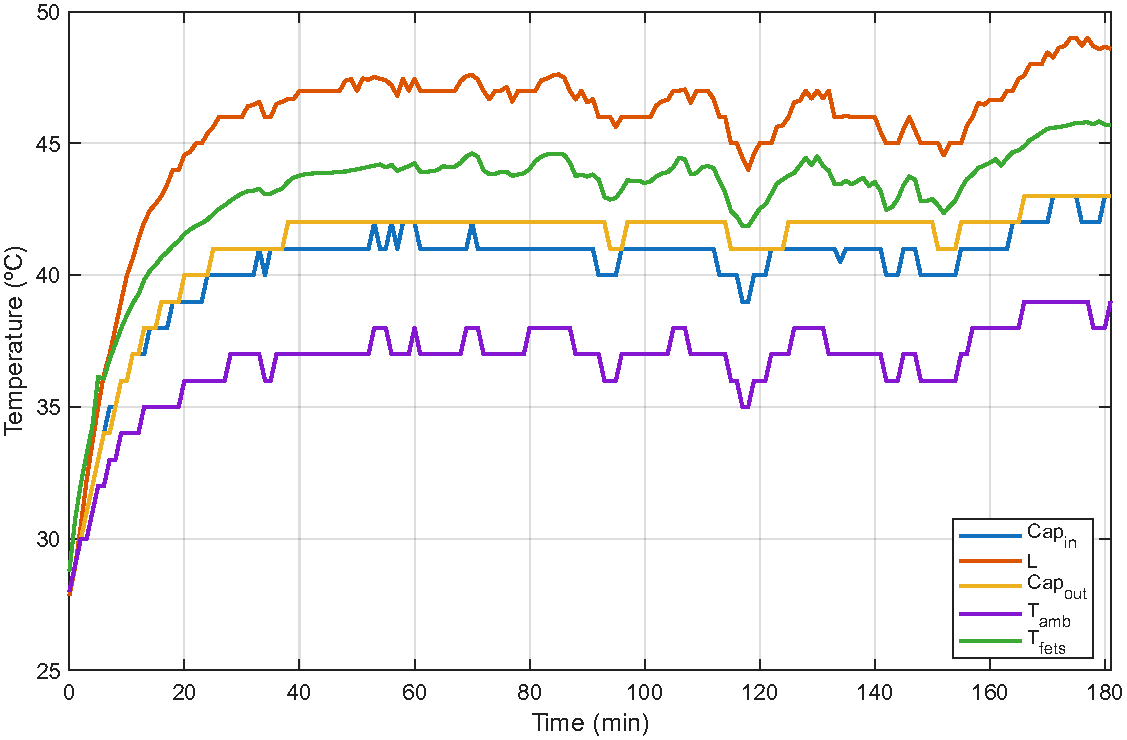
\includegraphics[width=0.6\linewidth]{Images/LAB_res/Temperatures vs time.pdf} 
            \caption{Temperature evolution during 3 hours.} 
            \label{fig:3h_temp_test}
        \end{figure} 
        
        From Figure~\ref{fig:3h_temp_test}, it can be concluded that after 40~min at maximum power, all the temperatures stop rising. Some oscillations were measured during the experiment due to the fact that ambient temperature also oscillated. As seen earlier the inductor is the element which heats the most, followed by the transistor and capacitors. After 3 hours, none of the elements reached a concerning temperature.

        With this test it is concluded that there is no need for cooling. At least in the same conditions of the test. To confirm this statement, the board was placed inside a cardboard box since \ac{tsb} usually places boards inside close boxes. If the components inside the box need cooling, a fan or a water cooling needs to be added.

        \begin{figure}[!ht] 
            \centering 
            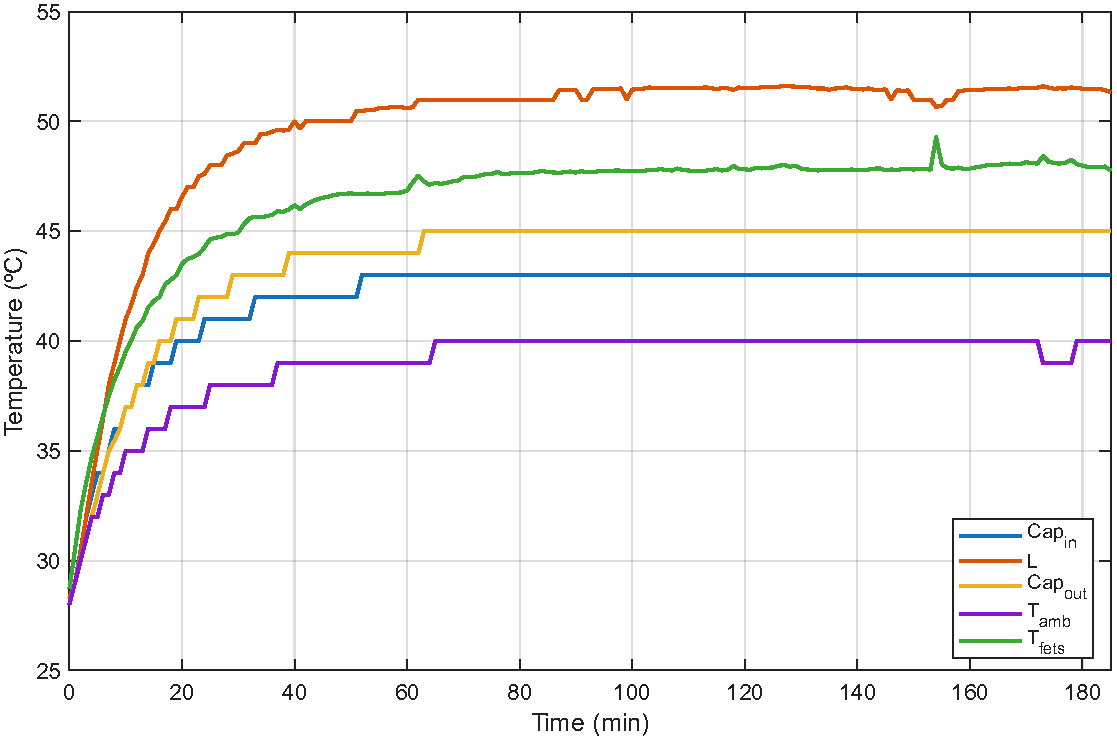
\includegraphics[width=0.6\linewidth]{Images/LAB_res/Temperatures_vs_time_close box.pdf} 
            \caption{Temperature evolution during 3 hours in a close box.} 
            \label{fig:3h_temp_test}
        \end{figure} 

        In Figure~\ref{fig:3h_temp_test} is represented the described test. Since there is no air flow, the ambient temperature reading is more stable and therefore the others too. As in the previous test, after 60 minutes the temperatures remained approximately constant and the maximum temperature was 51.6ºC. Since none of the temperatures show concerning values, it is safe to conclude that no additional cooling is needed


\section{MPPT}
    In this section the charging sate machine is tested as well as the \ac{mppt} algorithm to ensure the functionality of the prototype.

    In the following tests a laboratory setup was used, where a power supply (the SM 1500-CP-30) was used with an internal function which can simulate the behavior of a solar panel. This function was configured as a 35 cells solar panel at 25ºC and variable irradiance controlled by sending TCP messages. 

    The load was the battery from \ac{sr03}, which is described in section~\ref{sec:battery}.

    This setup ensures a controlled environment where the solar panel works at a specified temperature and irradiance parameters increasing the number of controlled variables. Since the environment conditions are set by the user, this setup can be easily replicated for future comparisons and therefore increasing the scientific value of the tests.

    \subsection{Efficiency}
        To validate the efficiency of the converter over different current and voltage inputs, an irradiance sweep was performed with $10~w/m^2$ steps from $100~w/m^2$ to $1000~w/m^2$. Each irradiance level is maintained over 2 seconds to ensure that the algorithm is stable. All the values measured during this time are used to perform an average. Additionally, outliers were removed for better results. 

        The result is an efficiency curve (Figure~\ref{fig:eff over current}) that increases with both the input current and the irradiance, which are approximately proportional. Since the test was performed with different solar panel parameters, three curves were obtained. The converter is clearly more efficient at higher input voltages, that is, for panels with more cells in series.

        \begin{figure}[!ht] 
            \centering 
            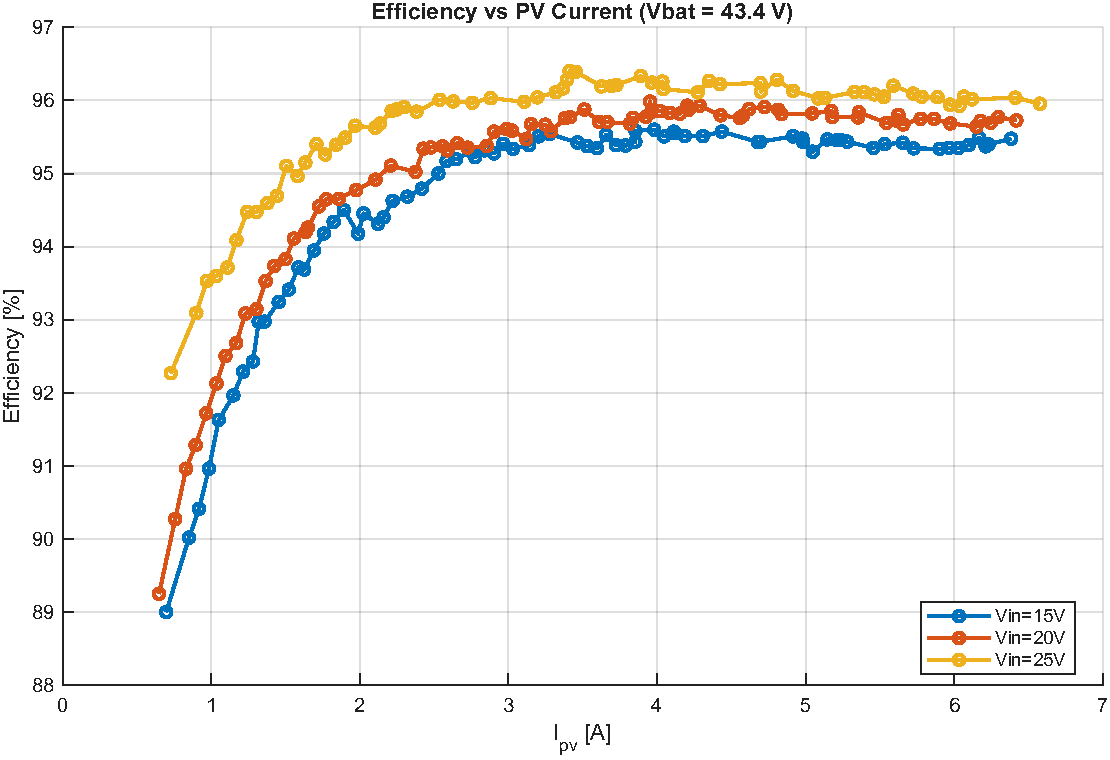
\includegraphics[width=0.6\linewidth]{Images/LAB_res/eff_ipv.pdf} 
            \caption{Converter efficiency over different input currents and voltages.} 
            \label{fig:eff over current}
        \end{figure}

        Both trends are expected. At low currents the efficiency is lower because the constant losses required to power the electronics (\ac{mcu}, sensors, etc.) have a larger relative impact. As the current increases, those losses become less significant and the efficiency stabilizes. After around 3 A, the converter switching losses become dominant. Since they increase with the input current, a slight downward slope of the curve is expected.

        The higher efficiency at higher input voltage is explained by the fact that a boost converter is more efficient at lower duty cycles. From equation \ref{eq:duty}, for a given output voltage the duty cycle decreases as the input voltage increases. Therefore, increasing the number of cells in series reduces the duty cycle and improves the efficiency.

        On the other hand, if the input voltage is constant and the output voltage increases (Figure~\ref{fig:eff over output voltage}), the efficiency will reduce due to the same reason. Equation \ref{eq:duty} tells us that for a fix input voltage the duty cycle will increase and therefore the efficiency will decrease.   

        \begin{figure}[!ht] 
            \centering 
            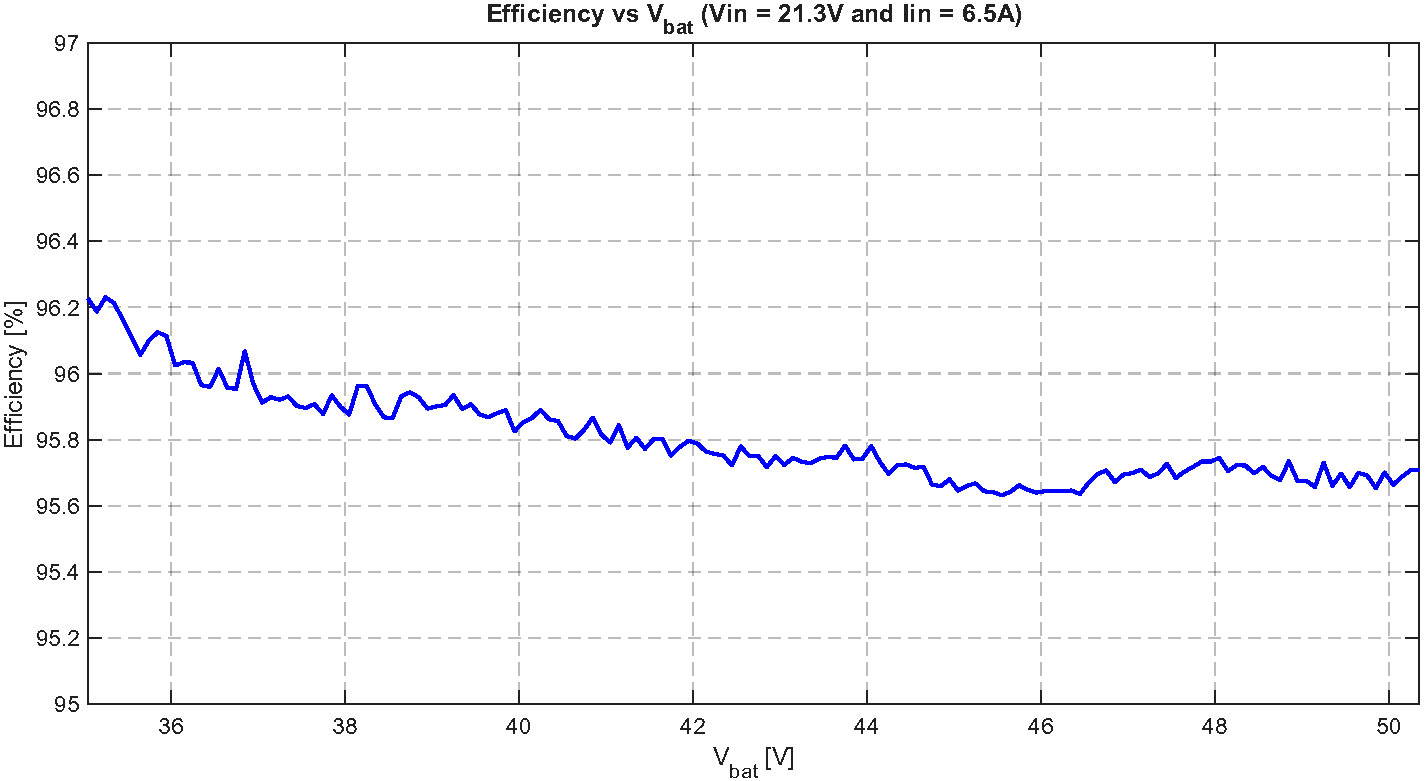
\includegraphics[width=0.6\linewidth]{Images/LAB_res/eff_vout.pdf} 
            \caption{Converter efficiency over output voltage.} 
            \label{fig:eff over output voltage}
        \end{figure}


    \subsection{Tracking speed}
        Several configurations were tested to optimise the \ac{peo} algorithm. Following the tuning process, the final configuration was defined as shown in Table~\ref{tab:MPPT_config}.

        \begin{table}[!ht]
        \centering
        \caption{MPPT parameters.}
        \label{tab:MPPT_config}
            \begin{tabular}{|c|c|c|c|}
            \hline
            Sampling frequency & MPPT frequency & Step size & Power Dead Band \\
            \hline
            1~kHz & 50~Hz & 0.7~\% & 700~mW \\
            \hline
            \end{tabular}
        \end{table}

        To evaluate the performance of the \ac{mppt} algorithm under varying environmental conditions, several Python scripts were developed to control the temperature and irradiance of the power source. Through a LAN connection, the scripts transmit TCP messages to the power supply, allowing its environmental parameters to be modified during the tests.

        Two test scenarios were defined:

        \begin{enumerate}
            \item \textbf{Irradiance staircase:} The test starts at an irradiance of 1000~$\mathrm{W/m^2}$, which is subsequently reduced by 200~$\mathrm{W/m^2}$ at approximately 2~s intervals until reaching 200~$\mathrm{W/m^2}$. The irradiance is then increased using the same sequence until returning to 1000~$\mathrm{W/m^2}$.

            \item \textbf{Temperature staircase:} The test starts at 25~$^\circ$C, after which the temperature is increased in 10~$^\circ$C steps at 2~s intervals until reaching 85~$^\circ$C. The temperature is then decreased using the same sequence until returning to 25~$^\circ$C.
        \end{enumerate}

        Both tests were divided into two phases. In the first phase, the environmental parameters were varied gradually to evaluate the tracking performance under normal operating conditions. In the second phase, more abrupt changes were introduced to assess the tracking performance under more demanding conditions. This approach allows the response of the algorithm to be evaluated for both gradual and rapid variations in the operating conditions.

        The results of the irradiance and temperature staircase tests are presented in Figures~\ref{fig:irr_stairway} and \ref{fig:temp_stairway}, respectively. Overall, the algorithm demonstrated satisfactory tracking performance, maintaining the operating point close to the \ac{mpp} while responding to changes in the environmental conditions.


        \begin{figure}[!ht]
            \centering
            \begin{minipage}[b]{0.49\textwidth}
                \centering
                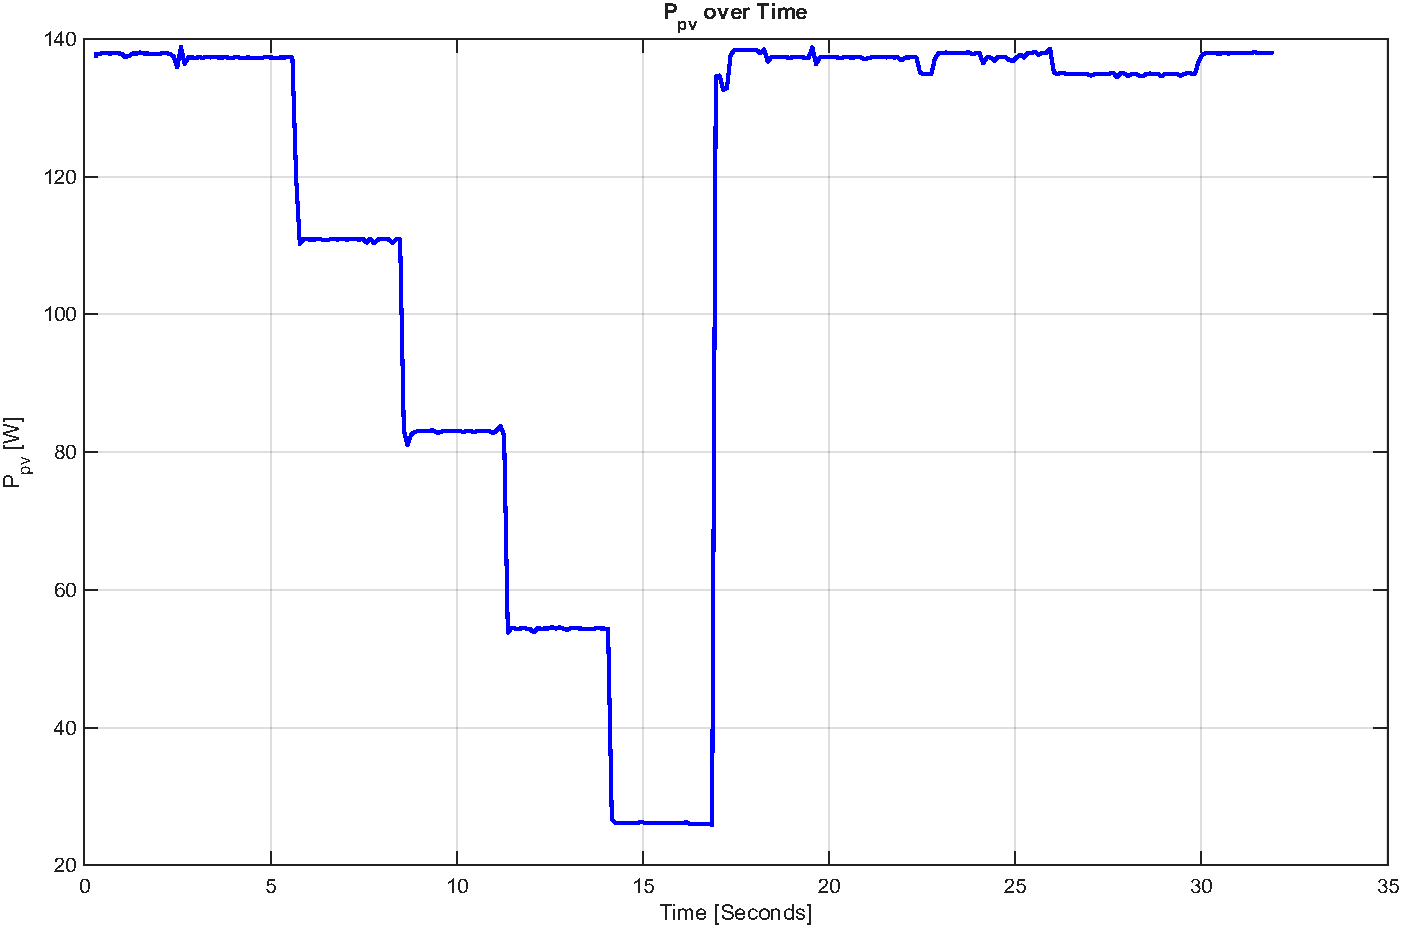
\includegraphics[width=\textwidth]{Images/LAB_res/irr_stairway.pdf}
                \caption{Power response for the "Irradiance stairway" test.}
                \label{fig:irr_stairway}
            \end{minipage}
            \hfill
            \begin{minipage}[b]{0.49\textwidth}
                \centering
                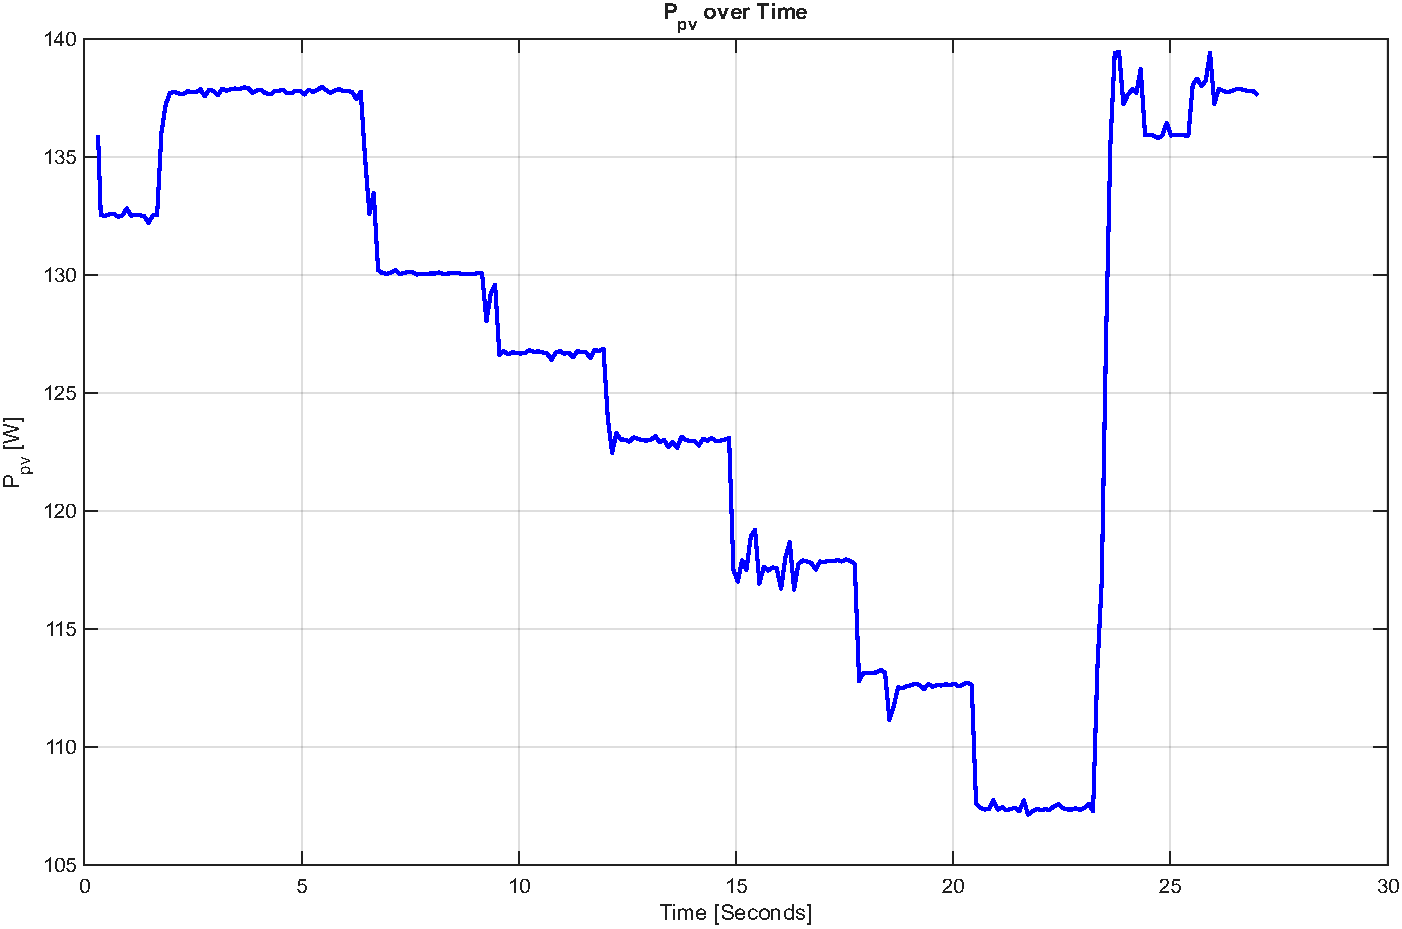
\includegraphics[width=\textwidth]{Images/LAB_res/temp_stairway.pdf}
                \caption{Power response for the "Temperature stairway" tes.}
                \label{fig:temp_stairway}
            \end{minipage}
        \end{figure}

        \textcolor{red}{Increase CAN send rate, crop the data, add reference lines.}

        For both tests, the tracking speed was measured and it is represented in table.

        \begin{table}[!ht]
            \centering
            \caption{Tracking speed (ms) for irradiance stairway test.}
            \label{tab:irr_stairway}
            \begin{tabular}{|c|c|c|c|c|}
                \hline
                 1000 to 800~$\mathrm{W/m}^2$ & 800 to 600~$\mathrm{W/m}^2$ & 600 to 400~$\mathrm{W/m}^2$ & 400 to 200~$\mathrm{W/m}^2$ & 200 to 1000~$\mathrm{W/m}^2$\\
                \hline
                 ? & ? & ? & ? & ?\\
                \hline 
            \end{tabular}
        \end{table}

        \begin{table}[!ht]
            \centering
            \caption{Tracking speed (ms) for temperature stairway test.}
            \label{tab:temp_stairway}
            \begin{tabular}{|c|c|c|c|c|c|c|}
                \hline
                 25 to 35ºC & 35 to 45ºC & 45 to 55ºC & 55 to 65ºC & 65 to 75ºC & 75 to 85ºC & 75 to 35ºC\\
                \hline
                 ? & ? & ? & ? & ? & ? & ?\\
                \hline 
            \end{tabular}
        \end{table}

        \textcolor{red}{analise}
        
        
    
\section{Field test}
    To prove the functionality of the developed prototype, two charging tests were recorded. Both tests use the smaller battery described in chapter~\ref{}.

    By using the SM 1500-CP-30 power supply in photovoltaic function connected to the \ac{mppt} charger, the battery was fully charged. Figure~\ref{fig:full charge in lab} shows the result where the CC-CV charging curve was accomplish. In \ac{cc} mode, the algorithm tracked the \ac{mpp} successfully. At \ac{cv}, the output voltage is constant, and the output current dropped slowly. 

    \textcolor{red}{O fim do teste está miseravel, era bom tentar corrigir isto e mostrar que o conversor entra em charge end}

    \begin{figure}[!ht] 
        \centering 
        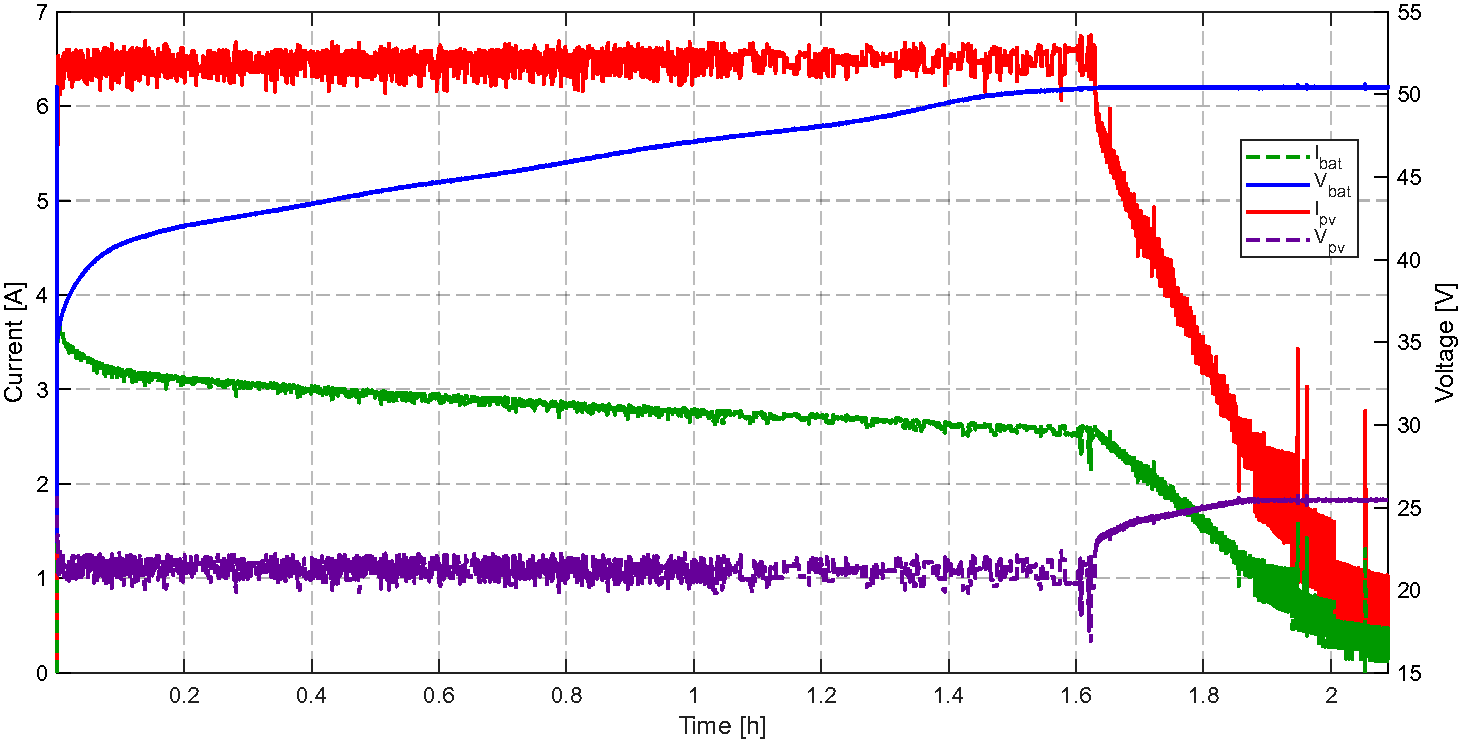
\includegraphics[width=0.8\linewidth]{Images/LAB_res/charging_test_lab.pdf} 
        \caption{Full battery charge in laboratory.} 
        \label{fig:full charge in lab}
    \end{figure} 


    Parei o teste duas vezes e é facilmente notavel no grafico. Em cerca de 3h 30min tive de mudar de sitio pq fiquei sem sol. Perto das 6h percebi que os paineis não estavam a operar em MPP devido a uma limitação do duty cycle maximo que aconteceu pela primeira vez devido ao painel ser muito pequeno.

    The last test is a field test with a solar panel of 20 cells submitted to the environment conditions. The test was stopped two times. The first one around 3.5h to change the test spot and the second around 5.45h to correct a mistake. At first the algorithm was never reaching \ac{mpp}, i though that was due to the solar panel temperature and therefore the solar panel was cooled with water several times during the test. Almost at the end, i realized that the duty cycle was reaching the limit imposed in firmware and therefore it was never reaching \ac{mpp}. This was never a problem since i had not tested the algorithm with such small solar panel. The rest of the test went as expected.
    
    \begin{figure}[!ht] 
        \centering 
        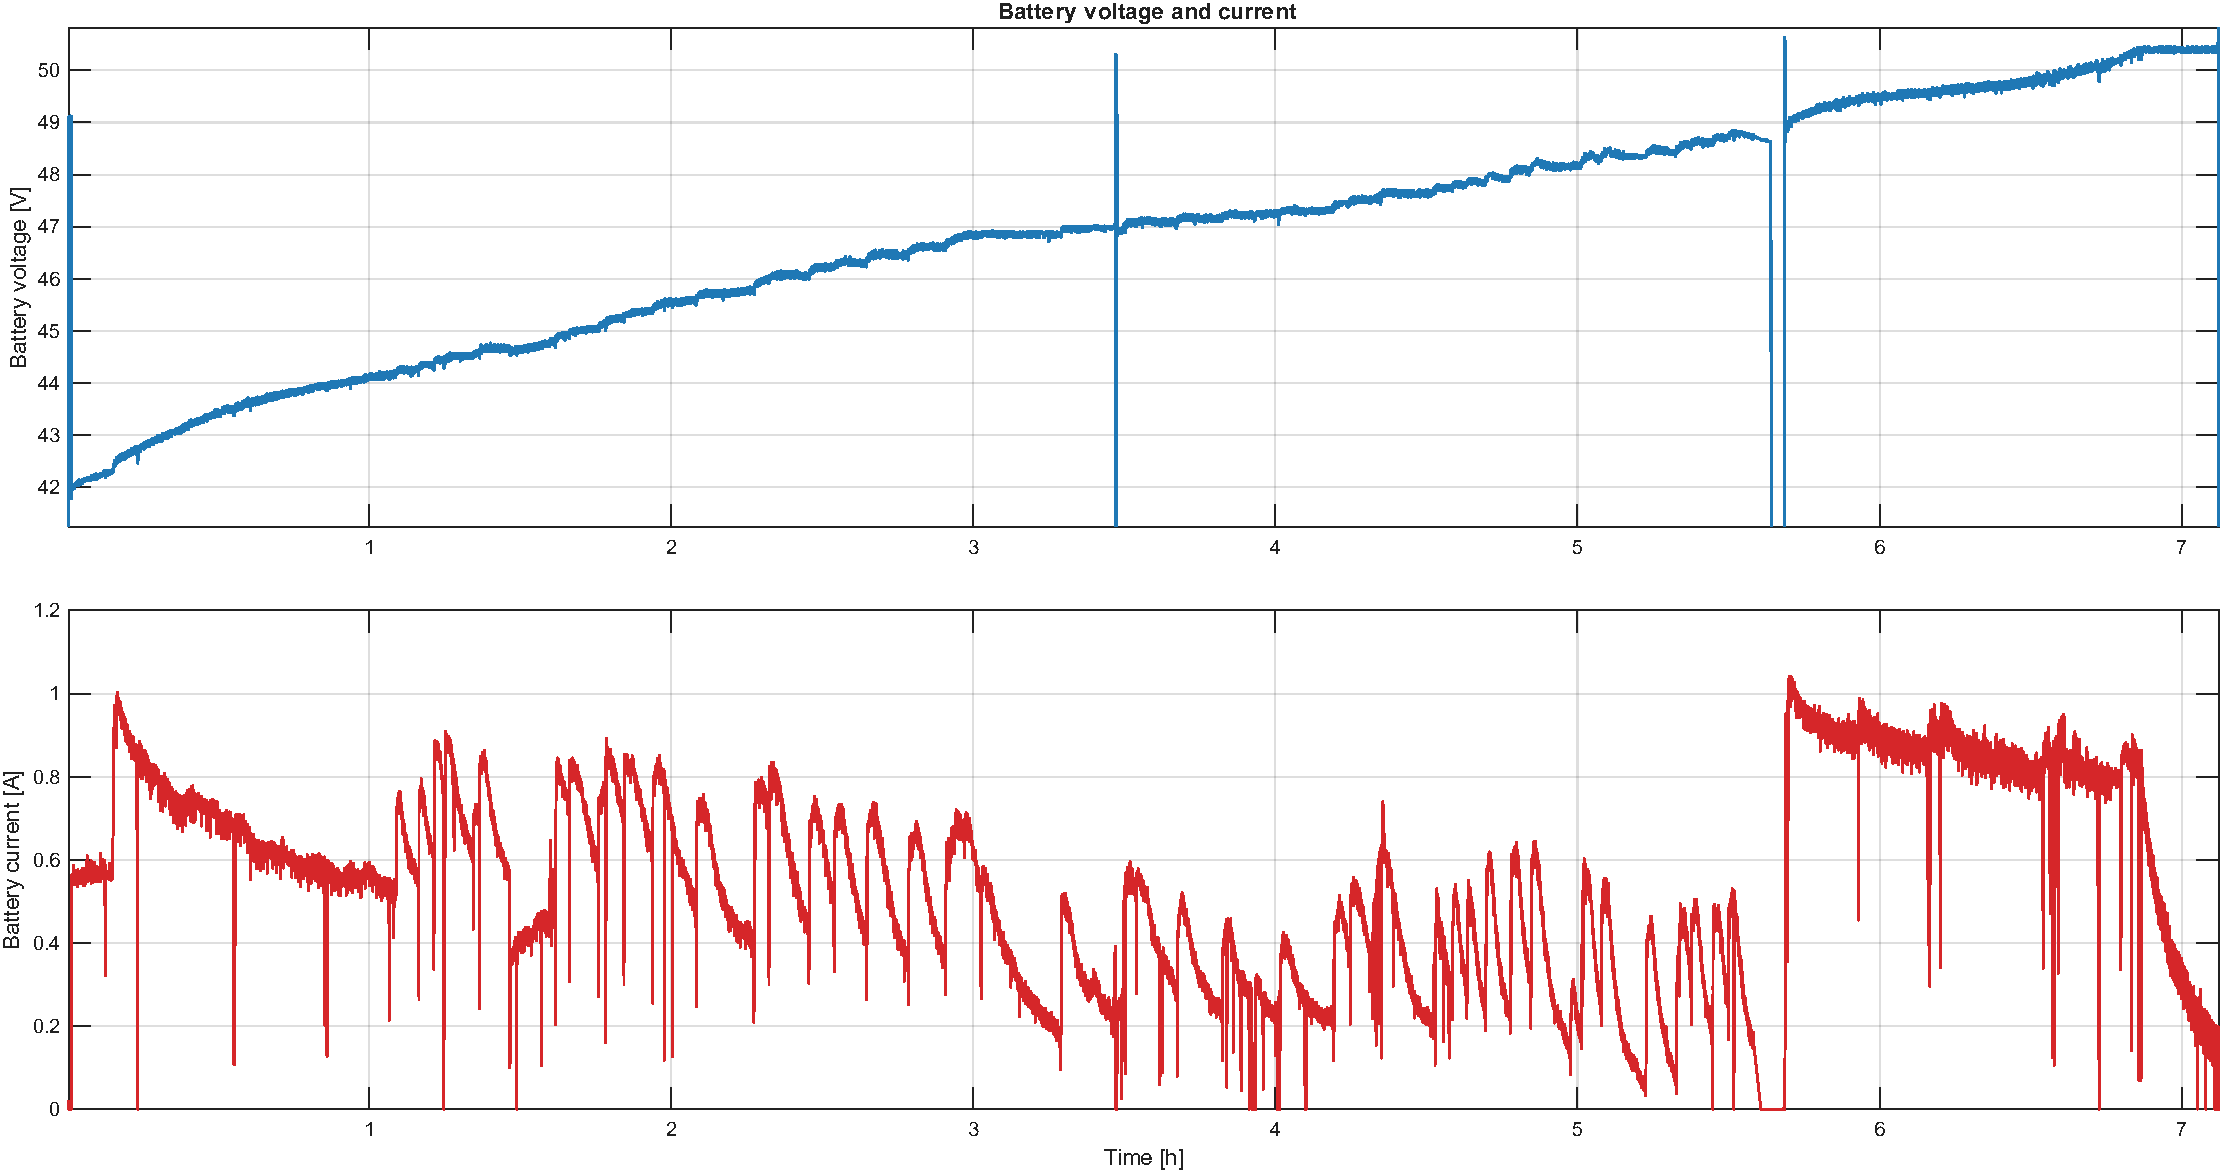
\includegraphics[width=0.8\linewidth]{Images/LAB_res/charging_test.pdf} 
        \caption{Battery charging test. Voltage and current curve.} 
        \label{fig:}
    \end{figure} 


        

        \textcolor{red}{Show the MPPT in difrent states. No load-Sweep-CC-CV-no load-CV-CC}

        \textcolor{red}{Repetir teste.}

        \textcolor{red}{Se possivel adicionar testes em água.}